\begin{center}
  \vspace*{25pt}
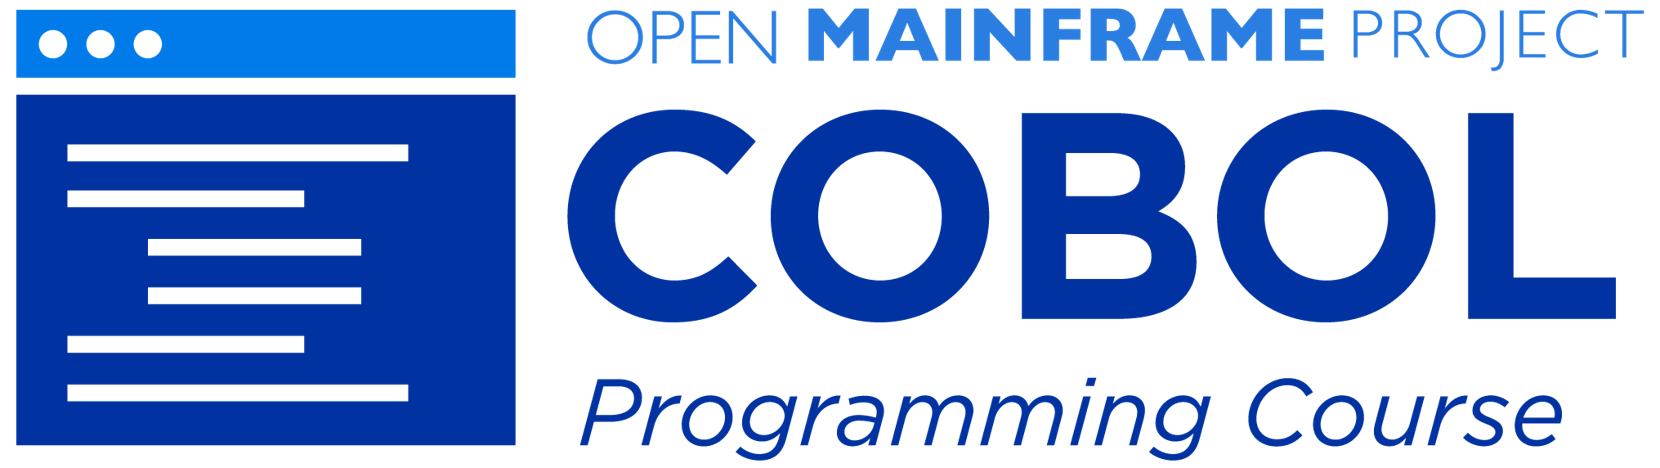
\includegraphics{Images/COBOL-Programming-Course.png}
\hypertarget{cobol-programming-course-1}{%
\section*{
  \\[35pt]
  \Huge Curso de Programación en COBOL 1 \\[10pt]
  \Huge Introducción \\[15pt]
  \Large Version 3.0.0}\label{cobol-programming-course-1}}
\end{center}

\pagebreak
\hypertarget{copyright}{%
\section*{Copyright}{
  \normalsize COBOL Programming Course is licensed under Creative Commons 
  Attribution 4.0 International. To view a copy of this license, visit 
  \href{https://creativecommons.org/licenses/by/4.0}{https://creativecommons.org/licenses/by/4.0}. \\[10pt]
  Copyright Contributors to the Open Mainframe Project's COBOL Programming Course}\label{copyright}}
\pagebreak

\hypertarget{preface}{%
\section*{Prefacio}\label{preface}}

\hypertarget{abstract}{%
\subsection*{Resumen}\label{abstract}}

Solamente un lenguaje de programación ha sido diseñado específicamente 
para aplicaciones empresariales, Common Business-Oriented Language, COBOL.
En la actualidad COBOL se mantiene tan relevante como antes, manejando
\$3 billones de dólares en comercio cada día.

Esta publicación está dirigida a principiantes que buscan aprender
de COBOL. Describe como trabajar con COBOL usando herramientas modernas
como Visual Studio Code, y extensiones como Zowe para Visual Studio Code
y z Open Editor. Además describe como escribir, probar, ejecutar y 
depurar programas escritos en COBOL.

\hypertarget{authors}{%
\subsection*{Autores}\label{authors}}

\textbf{Michael Bauer} Es un desarrollador líder para el desarrollo
del flujo de valor de Open Mainframe en Broadcom. Y dirige la iniciativa
de código abierto de Zowe. El entorno de desarrollo Zowe es una popular
herramienta para interactuar con z/OS, y abre la oportunidad a los 
trabajos hechos sobre sistemas Mainframe de usar la metodología DevOps
y sus prácticas. Mike lidera el equipo de desarrollo de la linea de comandos
de Zowe (Zowe CLI), quienes crearon y recientemente dieron a conocer el
explorador de Zowe, que es una extension para Visual Studio Code.
El tambien es un reconocido orador y blogger, y ha realizado talleres
interactivos alrededor del mundo para aquellos interesados en incorporar
los sistemas Mainframe en sus actividades de DevOps.

\textbf{Ahmed Eid} Es un estudiante de ingeniería de sistemas en Egipto.
Además, él fue un alumno de la mentoría realizada en el verano de 2021,
y estuvo organizada por Open Mainframe Project. 
Y colaboro para mejorar el contenido del curso de programacion en COBOL.

\textbf{Zeibura Kathau} Se desempeña como un escritor técnico para el equipo
de generación de valor de los mainframe utilizando tecnologías DevOps para Broadcom.
Y ha trabajado en proyectos de código abierto como Che4z y Code4z, que son extensiones
de IDEs dirigida a desarrolladores de sistemas mainframe. Durante su recorrido el goza
de 8 años de experiencia en el área de tecnologías de la información.

\textbf{Makenzie Manna} Actualmente está trabajando como líder de IBM Redbooks
en los Estados Unidos. Ella lleva 3 años de experiencia en el área del desarrollo
de software, junto a su Máster en ciencias de la computación en la Universidad de Marist.
Sus areas de experiencia incluyen matemáticas, IBM Z y desarrollo en la nube.

\textbf{Paul Newton} Trabaja como consultor de IT en los Estados Unidos.
Y ha reunido 40 años de experiencia en el área de tecnologías de la información.
Es egresado de la Universidad de Arizona. Y sus áreas de experiencia son IBM Z,
z/OS, y LinuxONE. Y se ha dedicado a escribir software para tecnologías basadas en
z/OS.

\textbf{Jonathan Sayles} Ha trabajado como un educador técnico en IBM,
y es reconocido por ser seminarista y dictar cursos de entrenamiento para
diversas tecnologías. Ha acumulado más de 40 años en el sector de TI,
combinando tanto el área académica y corporativa. Además, se ha desempeñado
como desarrollador de software, diseñador, consultor y diversos otros
roles teniendo como foco bases de datos relacionales, IDE, y tecnologías
orientadas a objetos. Jonathan ha participado en la escritura de más de 16
libros t más de 150 artículos en Journals de carácter técnico. Asimismo
él es el coautor de "Informix 4GL to Enterprise Generation
Language (EGL)", SG24-6673 y de "z/OS Traditional Application Maintenance
and Support", SG24-7868.

\textbf{Hartanto Ario Widjaya} Es un estudiante de ciencias de la computación en
la Universidad de Gestion de Singapur. Fue un estudiante de la mentoría de verano
de la organización Open Mainframe, y estuvo trabajando en el curso de programación
en COBOL. Él estuvo interesado a mejorar el contenido del curso y en asistir
a personas en la incorporación de COBOL como parte de su tecnología de trabajo.

\textbf{William Yates} Es un ingeniero de software que trabaja para IBM UK.
En la mayor parte de su carrera él ha estado trabajando en CICS TS como
arquitecto de pruebas y como tester de software. Ha producido contenido técnico
para varias publicaciones de Redbooks como videos para cursos, y en conferencias
alrededor del mundo. Además, es uno de los lideres en el proyecto Galasa,
construyendo frameworks de integración de pruebas para sistemas de nube hibrida.
Para más información \href{https://galasa.dev/}{https://galasa.dev}.

\hypertarget{acknowledgements}{%
\subsection*{Agradecimientos}\label{acknowledgements}}

Especial gracias a quienes participaron en la residencia para darle forma a esta publicación.

\begin{itemize}
\item
  Dr.~Tak Auyeung, Profesor en American River College
\item
  Jeffrey Bisti, Arquitecto en el ecosistema Z, IBM
\item
  Ilicena Elliott, Especialista de IT II, Departamento de recursos humanos
\item
  Martin Keen, Técnico de servicios en contenido, IBM
\item
  Sudharsana Srinivasan, Influencer coordinador del programa Z, IBM
\item
  Suzy Wong, Especialista en tecnologías de la información, DMV
\item
  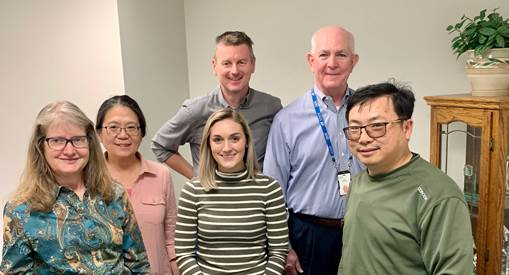
\includegraphics{Images/image004.jpg}
\end{itemize}

De izquierda a derecha: Ilicena, Suzy, Makenzie, Martin, Paul, y Tak
\pagebreak
